%!TEX root = panda.tex
%!TEX program = lualatex

\documentclass{easychair}
% !TeX root = design.tex
%!TEX program = lualatex


\usepackage[utf8]{inputenc}
\usepackage[T1]{fontenc}

\usepackage{fontspec}
\usepackage{lmodern}

% add page number
% \pagestyle{headings}

% beamer setting
% \usetheme{CambridgeUS}
% \setbeamertemplate{footline}[page number]
% \setbeamertemplate{blocks}[rounded][shadow=true]

% \pdfoptionpdfminorversion=7
% \pdfminorversion=6

% use table of content for each chapter
% \usepackage{minitoc}

% \usepackage[a-3u]{pdfx}

% \usepackage[toc,page]{appendix}
\usepackage[titletoc]{appendix}

% csquotes
\usepackage{csquotes}

% use biblatex
\usepackage[sorting=anyt,sortcites=true,backend=biber,url=false,doi=false,maxnames=7,isbn=false,firstinits=true,style=numeric]{biblatex}
% \addbibresource{reference}
\bibliography{reference}


% encoding (just for pdflatex)
% \usepackage[latin1]{inputenc}

% hyphenating
\usepackage[english]{babel}
% \usepackage[autostyle]{csquotes}

% AMS Math
\usepackage{braket}
% \usepackage{amsmath,amssymb,amsthm,mathtools}
% \usepackage{breqn}
\usepackage{amsmath,amssymb,mathtools,amsthm}
% \usepackage{unicode-math}
% \usepackage{lualatex-math}
% \usepackage{stix}
% \usepackage{cmbright}
% \usepackage{lmodern}
% \usepackage{lxfonts}
\usepackage{nicefrac}
\usepackage{stmaryrd}
\usepackage{xfrac}
% \usepackage{MnSymbol}


% for algorithm
%\usepackage{algorithm}
%\usepackage{algpseudocode}
\usepackage{algorithm2e}
\SetAlFnt{\small}

% hyperref
\usepackage{hyperref}
% \usepackage[pdfa]{tulhypref}
\hypersetup
{
%   bookmarks       = true,
  unicode         = true,
  pdftitle        = Maze challenge,
  pdfauthor       = Verimag, %auteur du document
  pdfsubject      = Maze challenge,
  pdftoolbar      = true, %barre d'outils non visible
  pdfmenubar      = true, %barre de menu visible
  pdfhighlight    = /O, %effet d'un clic sur un lien hypertexte
  colorlinks      = true, %couleurs sur les liens hypertextes
%   pdfpagemode = None, %aucun mode de page
%   pdfpagelayout = SinglePage, %ouverture en simple page
  pdffitwindow    = true, %pages ouvertes entierement dans toute la fenetre
  linkcolor       = violet, %couleur des liens hypertextes internes
  citecolor       = blue, %couleur des liens pour les citations
  urlcolor        = orange, %couleur des liens pour les url
%   pagebackref=true
%   bookmarksdepth  = 3
}

% \usepackage[sc]{mathpazo}
% \newfontfamily\DejaSans{DejaVu Sans}

\usepackage[usenames,dvipsnames,svgnames,table]{xcolor}
\definecolor{darkgoldenrod}{rgb}{0.72, 0.53, 0.04}
\definecolor{darkorchid}{rgb}{0.6, 0.2, 0.8}
% for listings
\usepackage{listings}
\lstset{basicstyle=\footnotesize\ttfamily,showspaces=false,frame=tb}
% \ltset{basicstyle=\small\ttfamily,showspaces=false,frame=tb}
\lstloadlanguages{C++,[x86masm]Assembler}

% graphicx and caption
\usepackage{graphicx}
% \usepackage{bmpsize}
% \usepackage[font={small}]{caption}
\usepackage{caption}
% \usepackage{subfig}
% \usepackage[config,position=t]{subfig}
\usepackage{subcaption}
% \captionsetup{compatibility=false}
% \DeclareCaptionLabelSeparator{periodspace}{.\quad}
% \captionsetup{font=footnotesize,labelsep=periodspace,singlelinecheck=false}
% \captionsetup[sub]{font=footnotesize,singlelinecheck=true}
% \renewcommand\thesubfigure{(\alph{subfigure})}
% \usepackage{rotating}
\usepackage{pdfpages}

% for smarter reference
\usepackage{cleveref}

% reference depth
\setcounter{secnumdepth}{2}

% for appendix
% \usepackage{appendix}

% for footnote
\usepackage{fancyvrb}
\VerbatimFootnotes

% for diagram
\usepackage{tikz}
\usetikzlibrary{calc,
                automata,
                arrows,
                matrix, 
                plotmarks,
                positioning,
                shapes,
                shapes.multipart,
                shapes.misc,
                decorations, 
                decorations.markings, 
                decorations.pathreplacing, 
                decorations.pathmorphing,
                backgrounds,
                fit,
                patterns}
% \usepackage{tkz-base}

% for commutative diagram
\usepackage{tikz-cd}
%\tikzset{commutative diagram/row}

\usepackage{wrapfig}

% for margin note
\usepackage{marginnote}

% for itemize
\usepackage{enumerate}
\usepackage[inline]{enumitem}
% \setitemize{label=\usebeamerfont*{itemize item}%
%   \usebeamercolor[fg]{itemize item}
%   \usebeamertemplate{itemize item}}

% create procedure environment
%\newtheorem{procedure}{Procedure}

% some tikz styles
% \tikzset{morphism/.style={circle,draw,thick,align=center,inner sep=0pt,minimum size=12pt}}
% \tikzset{bigmorphism/.style={circle,draw,thick,align=center,inner sep=0pt,minimum size=25pt}}
%\tikzset{objects/.style=}

% enumitem
% \usepackage{enumitem}

\usepackage{fancyvrb}

\usepackage{cprotect}

\usepackage{footmisc}

\usepackage{array}

% \usepackage{gnuplottex}

\usepackage{float}

\usepackage{mathrsfs}

\usepackage[export]{adjustbox}

\usepackage{rotating}

% for footnote
\usepackage{perpage} 
\MakePerPage{footnote}

\usepackage{parcolumns}

\usepackage{url}

% \usepackage{savetrees}

% \usepackage{floatrow}
% \floatsetup[table]{font=small}

% \newtheorem{principle}{Principle}
% \crefname{principle}{principle}{principles}
% \Crefname{principle}{Principle}{Principles}

\theoremstyle{plain}

% \newtheorem{hypothesis}{Hypothesis}
% \crefname{hypothesis}{hypothesis}{hypotheses}
% \Crefname{hypothesis}{Hypothesis}{Hypotheses}
% 
% \newtheorem{assumption}{Assumption}
% \crefname{assumption}{assumption}{assumptions}
% \Crefname{assumption}{Assumption}{Assumptions}
% 
% \newtheorem{heuristic}{Heuristic}
% \crefname{heuristic}{heuristic}{heuristics}
% \Crefname{heuristic}{Heuristic}{Heuristics}


\newtheorem{theorem}{Theorem}
\crefname{theorem}{theorem}{theorem}
\Crefname{theorem}{Theorem}{Theorems}

% \newtheorem{proposition}{Proposition}[section]
\newtheorem{proposition}{Proposition}
\crefname{proposition}{proposition}{propositions}
\Crefname{proposition}{Proposition}{Propositions}
% 
\newtheorem{corollary}{Corollary}[section]
\crefname{corollary}{corollary}{corollaries}
\Crefname{corollary}{Corollary}{Corollaries}

\newtheorem{problem}{Problem}
\crefname{problem}{problem}{problems}
\Crefname{problem}{Problem}{Problems}

\newtheorem{lemma}{Lemma}[section]
\crefname{lemma}{lemma}{lemmas}
\Crefname{lemma}{Lemma}{Lemmas}

\newtheorem{observation}{Observation}[section]
\crefname{observation}{observation}{observations}
\Crefname{observation}{Observation}{Observations}

\theoremstyle{definition}
% 
\newtheorem{definition}{Definition}[section]
\crefname{definition}{definition}{definitions}
\Crefname{definition}{Definition}{Definitions}
% 
\newtheorem{hypothesis}{Hypothesis}
\crefname{hypothesis}{hypothesis}{hypotheses}
\Crefname{hypothesis}{Hypothesis}{Hypotheses}

% \newtheoremstyle{dotlessP}{}{}{}{}{\color{blue}\bfseries}{}{ }{}

% \theoremstyle{dotlessP}
% \theoremstyle{plain}
\theoremstyle{remark}

% \newtheorem{example}{Example}[section]
\newtheorem{example}{Example}
\crefname{example}{example}{examples}
\Crefname{example}{Example}{Examples}

\theoremstyle{remark}

% \newtheorem{remark}{Remark}[section]
\newtheorem{remark}{Remark}
\crefname{remark}{remark}{remarks}
\Crefname{remark}{Remark}{Remarks}

\newtheorem{note}{Note}[section]
\crefname{note}{note}{notes}
\Crefname{note}{Note}{Notes}

\crefname{secinapp}{appendix}{appendices}
\Crefname{secinapp}{Appendix}{Appendices}

% \crefname{appendix}{appendix}{appendices}
% \Crefname{appendix}{Appendix}{Appendices}
% \newtheorem{corollary}{Corollary}

% \newtheoremstyle{dotlessP}{}{}{}{}{\color{blue}\bfseries}{}{ }{}
% \theoremstyle{dotlessP}

%%%% BINARY INSTRUCTION %%%%
% \newcommand{\jump}{{\tt jump}\xspace}
% \newcommand{\call}{{\tt call}\xspace}
% \newcommand{\ret}{{\tt ret}\xspace}
% \newcommand{\jcc}{{\tt jcc}\xspace}
% \newcommand{\instr}{{\tt i}\xspace}
% \newcommand{\code}{{\tt c}\xspace}
% 
% %%%% GENERAL %%%%%%%%%%
% \newcommand{\dcfg}[1]{{\cal G}_{#1}}
% \newcommand{\E}{{\cal E}}
% \newcommand{\V}{{\cal V}}
% % \newcommand{\T}{{\cal T}}
% \newcommand{\N}{{\mathbb{N}}}

% \newtheorem{problem}{Problem}
% \crefname{problem}{problem}{problems}
% \Crefname(problem}{Problem}{Problems}

% \makeatletter
% \let\@twosidetrue\@twosidefalse
% \let\@mparswitchtrue\@mparswitchfalse
% \makeatother

% \usepackage[left=0.5cm,right=0.5cm,top=0.5cm,bottom=0.5cm]{geometry}

% \vspace{-2.5mm}
% \setlength{\textfloatsep}{\baselineskip plus 0.2\baselineskip minus 0.2\baselineskip}
% \setlength{\textfloatsep}{10pt}
% \setlength{\belowcaptionskip}{-10pt}
% \setlength{\intextsep}{10pt}
% \setlength\abovedisplayskip{0pt}
% \usepackage[font=small,skip=10pt]{caption}
\allowdisplaybreaks

% \usepackage{titlesec}
% \titlespacing\section{0pt}{12pt plus 4pt minus 2pt}{0pt plus 2pt minus 2pt}

% \setlength{\parindent}{0pt}
% \usepackage[nodisplayskipstretch]{setspace}
% \setstretch{1.5}

% \definecolor{cornflowerblue}{rgb}{0.39, 0.58, 0.93}

% \usepackage{lmodern}
% \usepackage[sc]{mathpazo}
% \linespread{1.05}
% \usepackage{baskervald}
% \usepackage{nbaskerv}
% \usepackage[utf8]{inputenc}
% \usepackage[T1]{fontenc}
% \usepackage{luatextra}
% \defaultfontfeatures{Ligatures=TeX}

% \usepackage{unicode-math}
% \usepackage{lualatex-math}
% \usepackage{charter}
% \usepackage[expert]{mathdesign}

\usepackage{afterpage}
\usepackage{changepage}

\usepackage{minted}
\usemintedstyle{friendly}
\usepackage{tcolorbox}
\usepackage{etoolbox}
% \BeforeBeginEnvironment{minted}{\begin{tcolorbox}}%
% \AfterEndEnvironment{minted}{\end{tcolorbox}}%

% \setcounter{totalnumber}{1}
% \setcounter{topnumber}{1}
% \setcounter{bottomnumber}{1}
% \renewcommand{\topfraction}{.99}
% \renewcommand{\bottomfraction}{.99}
% \renewcommand{\textfraction}{.01}

% \makeatletter
% \newcommand*{\twopagepicture}[4]{%
%     \checkoddpage
%     \ifoddpage
%         \expandafter\@firstofone
%     \else
%         \expandafter\afterpage
%     \fi
%     {\afterpage{%
%     \if #1t%
%         \if #2p%
%             \thispagestyle{empty}%
%             \afterpage{\thispagestyle{empty}}%
%         \fi
%     \fi
%     \begin{figure}[#1]
%         \if #2p%
%             \if #1t%
%                 \vspace*{-\dimexpr1in+\voffset+\topmargin+\headheight+\headsep\relax}%
%             \fi
%         \fi
%         \if #1b%
%             \caption{#4}%
%         \fi
%         \makebox[\textwidth][l]{%
%         \if #2p\relax
%             \let\mywidth\paperwidth
%             \hskip-\dimexpr1in+\hoffset+\evensidemargin\relax
%         \else
%             \let\mywidth\linewidth
%         \fi
%         \adjustbox{trim=0 0 {.5\width} 0,clip}{\includegraphics[width=2\mywidth]{#3}}}%
%         \if #1b\else
%             \caption{#4}%
%         \fi
%         \if #2p%
%             \if #1b%
%                 \vspace*{-\dimexpr\paperheight-\textheight-1in-\voffset-\topmargin-\headheight-\headsep\relax}%
%             \fi
%         \fi
%     \end{figure}%
%     \begin{figure}[#1]
%         \if #2p%
%             \if #1t%
%                 \vspace*{-\dimexpr1in+\voffset+\topmargin+\headheight+\headsep\relax}%
%             \fi
%         \fi
%         \makebox[\textwidth][l]{%
%         \if #2p%
%             \let\mywidth\paperwidth
%             \hskip-\dimexpr1in+\hoffset+\oddsidemargin\relax
%         \else
%             \let\mywidth\linewidth
%         \fi
%         \adjustbox{trim={.5\width} 0 0 0,clip}{\includegraphics[width=2\mywidth]{#3}}}%
%         \if #2p%
%             \if #1b%
%                 \vspace*{-\dimexpr\paperheight-\textheight-1in-\voffset-\topmargin-\headheight-\headsep\relax}%
%             \fi
%         \fi
%     \end{figure}%
%     }}%
% }
% \makeatother

% \usepackage[usenames]{color}

% some tikz styles
\tikzset{morphism/.style={circle,draw,thick,align=center,inner sep=0pt,minimum size=12pt}}
\tikzset{bigmorphism/.style={circle,draw,thick,align=center,inner sep=0pt,minimum size=25pt}}

\usepackage{setspace}
% \onehalfspacing

\def \i {\texttt{i}}
\def \ti {\textnormal{\texttt{i}}}
\def \Buf {\texttt{Buf}}
\def \tB {\texttt{B}}
\def \tBuf {\textnormal{\texttt{Buf}}}
\def \Addrs {\texttt{Addrs}}
\def \Bytes {\texttt{Bytes}}
\def \tBytes {\textnormal{\texttt{Bytes}}}

\def \tH {\texttt{H}}
\def \tT {\texttt{T}}
\def \tP {\texttt{P}}
\def \tU {\texttt{U}}
\def \tE {\texttt{E}}
\def \tF {\texttt{F}}
\def \tR {\texttt{R}}
\def \tS {\texttt{S}}
\def \tA {\texttt{A}}
\def \tY {\texttt{Y}}
\def \tP {\texttt{P}}
\def \tW {\texttt{W}}
\def \tV {\texttt{V}}
\def \tC {\texttt{C}}
\def \tD {\texttt{D}}
\def \tL {\texttt{L}}
\def \tI {\texttt{I}}

\def \tLF {\texttt{\textbackslash n}}
\def \tCR {\texttt{\textbackslash r}}
\def \tSP {\texttt{SPACE}}

\def \cA {\mathcal{A}}
\def \cC {\mathcal{C}}
\def \cD {\mathcal{D}}
\def \cM {\mathcal{M}}
\def \cN {\mathcal{N}}
\def \cR {\mathcal{R}}

% styles copied from http://tex.stackexchange.com/questions/168314/how-to-use-latex-commands-to-draw-a-flowchart
% \tikzset{
%   decision/.style = {
%     diamond,
%     draw
%   }
% }

\tikzset{decision/.style = 
  {
    diamond, draw, text width=7em, text badly centered, inner sep=0pt
  }
}

\tikzset{block/.style=
  {
    rectangle, draw, text width=17em, text centered, rounded corners
  }
}

\tikzset{ablock/.style=
  {
    rectangle, draw, text width=10em, text centered, rounded corners
  }
}

\tikzset{bblock/.style=
  {
    rectangle, draw, text width=8em, text centered, rounded corners
  }
}

\tikzset{cblock/.style=
  {
    rectangle, draw, text width=20em, text centered, rounded corners
  }
}

\tikzset{sblock/.style=
  {
    rectangle, draw, fill=blue!25, text width=4em, text centered, rounded corners
  }
}

\tikzset{descr/.style = 
  {
    fill = white, inner sept = 2.5pt
  }
}

\tikzset{connector/.style = 
  {
    -latex, font = \scriptsize
  }
}

\tikzset{rectangle connector/.style = 
  {
    connector, to path={(\tikztostart) -- ++(#1,0pt) \tikztonodes |- (\tikztotarget)}, pos = 0.5
  }
}

\tikzset{rectangle connector/.default = -2cm}

\tikzset{straight connector/.style = 
  {
    connector, to path=--(\tikztotarget) \tikztonodes
  }
}

\begin{document}

\title{GreHack 2015 - Weak Up Panda}
\titlerunning{GreHack 2015 - Weak Up Panda}

\author{Thanh Dinh Ta\inst{1}}
\authorrunning{Thanh Dinh Ta}

\institute{Verimag}

\clearpage
\maketitle

\section{Reversing}
The challenge is a $64$ bit ELF binary, when executes, it prints \texttt{badboy} and quits. A quick analysis with \texttt{ltrace} reveals that it reads an environment variable named \texttt{INPUT} (cf.~\Cref{fig:unset_input}). So we try to set a value for this variable (our shell is \texttt{fish}\footnote{\url{http://fishshell.com/}}):
\begin{lstlisting}[frame=lines, caption={Setting \texttt{INPUT}}, captionpos=b, boxpos=b, language=bash, label=lst:keygen]
set -x INPUT abcdef
\end{lstlisting}
and execute the crackme again (cf.~\Cref{fig:set_input}); still \texttt{badboy} though. There is no useful information yet, except that there are two \texttt{rand} calls, each followed by a \texttt{malloc}, maybe for storing the returned values of \texttt{rand}(s) (?); but we are not sure at this step \smiley{}.

\begin{figure}[ht]
  \centering
  \begin{subfigure}[b]{0.5\textwidth}
    \centering
    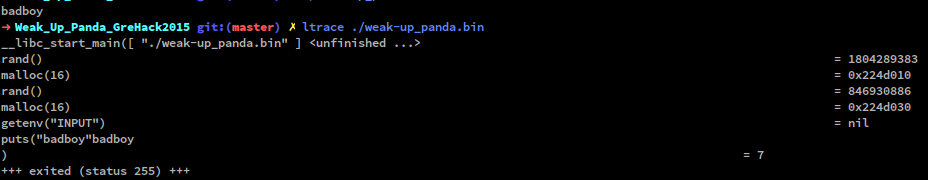
\includegraphics[width=0.9\textwidth,keepaspectratio]{ltrace_check.png}
    \caption{INPUT is unset}\label{fig:unset_input}
  \end{subfigure}%
  \begin{subfigure}[b]{0.5\textwidth}
    \centering
    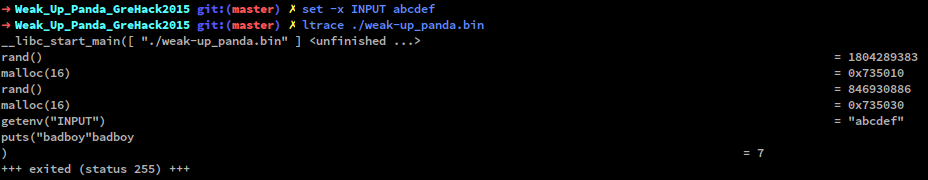
\includegraphics[width=0.9\textwidth,keepaspectratio]{ltrace_check_with_input.png}
    \caption{INPUT is set}\label{fig:set_input}
  \end{subfigure}
  \caption{Executing crackme with unset/set \texttt{INPUT}}
\end{figure}

We take a more detail analysis by drop this crackme into \texttt{IDA}, the \texttt{main} function can be quickly recognized from the familiar pattern: looking from the entry point, the address of \texttt{main} is passed as the first parameter for \texttt{libc\_start\_main}; here this address is \texttt{0x41806c}. At the first look, the structure of \texttt{main} seems simple, but it is not. The nightmare is from functions called by \texttt{main}: any of them has a \emph{tail call} to another function, and this called function, in its turn, has also tail to another one, so on and so forth; we even cannot believe into our eyes when seeing the function call graph generated by \texttt{IDA} \frownie{}. By searching for string ``badboy'', we also find the string ``goodboy'' and where it will be printed: this is at the function at \texttt{0x42e512}; more interesting this is called from a good/bad decision function at \texttt{0x41ce4a}.

We try next to run the crackme step-by-step, but give up soon since it is too long; the semantics of most functions (in this calling chain) are quite simple, then they do not give useful information. Moreover, many of them have exactly the same instructions (this is obviously a code redundancy but we do not understand why the crackme does that). This crackme maybe has intention to push the idea of \emph{continuation passing style} to the extreme\footnote{\url{https://en.wikipedia.org/wiki/Continuation-passing_style}}.

\paragraph{Black-box analysis}
The manual analysis with IDA does not work well, so we try our Pintool of BinSec project~\autocite{binsec}: this tool has capability of tracing only instructions executed in a range of addresses (here we set them as the first and the last address of \texttt{main}: \texttt{0x41806c} and \texttt{0x4181f6}), and tracing only internal instructions of the crackme (i.e.~the instructions of external calls \texttt{rand}, \texttt{malloc}, etc will be not counted). The following sequence shows the numbers of executed instructions where lengths of \texttt{INPUT} is $1, 2, 3, 4, 5, 6, 7, 8$:
\begin{equation*}
  51886, 66187, 80511, \dots, 137771, 168055
\end{equation*}
and if the length of \texttt{INPUT} is superior than $8$ then the corresponding number of executed instructions is always $168055$. The first $7$ numbers form an arithmetic progression with the difference $14301$, but the difference between $7$th to $8$th is $30284$. These observations suggest that the good \texttt{INPUT} should either have the length $8$ or the crackme does examine only $8$ first characters of \texttt{INPUT}). Since the number of executed instructions is stable for lengths superior than $8$ then we bias in favour the idea that there are only $8$ first characters are examined. Considering the numbers of excuted instructions as a \emph{program specification} for synthesizing~\autocite{GulwaniPPDP102}, we can give first an \emph{interpretation} for the crackme:
\begin{lstlisting}[frame=lines, caption={Synthesizing of the crackme}, captionpos=b, boxpos=b, language={C}, label=lst:synthesis]
for (i = 0; i < 8; ++i) {
  if (INPUT[i] == 0) return badboy();
  else fun_xxx(...);
}
if validate_xxx(INPUT, ...) then return goodboy();
else return badboy();
\end{lstlisting}
It might be worth noticing that this interpretation is valid for the observed constraints between values of \texttt{INPUT} and corresponding numbers of executed instructions; but it must be refined (by observing more information) to know whichs values will make the crackme print \texttt{goodboy}. Besides, the interpretation could be invalidated, for example when more information is observed. In both cases, more detail analysis must be carried. 

\section{Obfuscation elimination}
We now focus on values of \texttt{INPUT} with length $8$, but the number of executed instructions for this length is $168055$, manually examining such amount of instructions is not a good idea \smiley{}. Moreover, by manually examining several functions with IDA, we observe that most of them do not compute anything, and  many of them are even  identical!!!. One way to filter out such irrelevant instructions is to compare the execution traces result in from different values of \texttt{INPUT}: the irrelevant instructions should be the same between traces. We choose, for example, ``abcdefgh'' and ``HGFEDCBA'', the differences between two traces (generated by our Pintool) disclosure how the crackme work. For example, the first difference shown in~\Cref{fig:difference} reveals how the crackme checks whether a character is \texttt{NULL} or not.
% ; and \emph{understand immediately how the crackme works}.

\begin{figure}[ht]
  \centering
  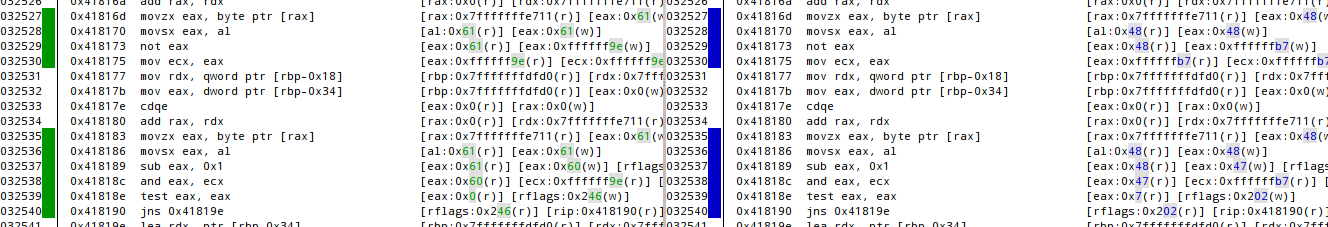
\includegraphics[width=0.75\textwidth,keepaspectratio]{difference.png}
  \caption{Differential analysis}\label{fig:difference}
\end{figure}

Literally, each character of the input is consumed by a loop which starts from \texttt{0x4181b5} (and backs to this address by a \texttt{leave} instruction). The intepretation that the crackme examines only first $8$ characters of \texttt{INPUT} (cf.~\Cref{lst:synthesis}) is validated by the following instructions (the order of current examined character is stored in \texttt{[rbp - 0x34]}) executed in each loop:
\begin{lstlisting}[frame=lines, caption={Checking if length is $8$}, captionpos=b, boxpos=b, language={[x86masm]Assembler}, label=lst:checklength]
0x4181b5  mov eax, dword ptr [rbp-0x34]
0x4181b8  and eax, 0xfffffff7
0x4181bb  mov edx, eax
0x4181bd  mov eax, dword ptr [rbp-0x34]
0x4181c0  xor eax, 0xfffffff7
0x4181c3  mov ecx, eax
0x4181c5  mov eax, dword ptr [rbp-0x34]
0x4181c8  sub eax, 0x8
0x4181cb  and eax, ecx
0x4181cd  or eax, edx
0x4181cf  test eax, eax
\end{lstlisting}
The computation on each character is dispersed over only several instructions (among $14586$ instructions of each loop) but it is direct to recognize them by observing only the differences between two traces. For example, the crackme uses unusual codes to check whether a character is \texttt{NULL} or not (cf.~\Cref{lst:checknull}; the character is stored in \texttt{[rax]}). We note that there are several irrelevant instructions between \texttt{0x418175} and \texttt{0x418183}.
 % (maybe for an obfuscation purpose \smiley{})
\begin{lstlisting}[frame=lines, caption={Checking if character is \texttt{NULL}}, captionpos=b, boxpos=b, language={[x86masm]Assembler}, label=lst:checknull]
0x41816d  movzx eax, byte ptr [rax]
0x418170  movsx eax, al
0x418173  not eax
0x418175  mov ecx, eax
...
0x418183  movzx eax, byte ptr [rax]
0x418186  movsx eax, al
0x418189  sub eax, 0x1
0x41818c  and eax, ecx
0x41818e  test eax, eax
\end{lstlisting}

\paragraph{Checksum algorithm}
In each loop, a character of \texttt{INPUT} and an additional value are used to calculate a checksum; this checksum is used as the additional value for the next loop. In summary, the checksum is calculated by:
\begin{lstlisting}[frame=lines, caption={Calculating checksum}, captionpos=b, boxpos=b, language={[x86masm]Assembler}, label=lst:checksumcalculation]
\end{lstlisting}
then is verified by (see also~\Cref{lst:checksumverificationcode}):
\begin{lstlisting}[frame=lines, caption={Verifying checksum}, captionpos=b, boxpos=b, language={[x86masm]Assembler}, label=lst:checksumverification]
\end{lstlisting}

\begin{lstlisting}[frame=lines, caption={Instructions verifying checksum}, captionpos=b, boxpos=b, language={[x86masm]Assembler}, label=lst:checksumverificationcode]
0x41d74f  mov rdx, qword ptr [rax]
0x41d752  mov rax, 0x122d4d05a4299633
0x41d75c  lea rcx, ptr [rdx+rax*1]
0x41d760  mov rax, qword ptr [rbp-0x8]
0x41d764  mov rdx, qword ptr [rax]
0x41d767  mov rax, 0x122d4d05a4299633
0x41d771  add rax, rdx
0x41d774  sar rax, 0x3f
0x41d778  xor rcx, rax
0x41d77b  mov rax, qword ptr [rbp-0x8]
0x41d77f  mov rdx, qword ptr [rax]
0x41d782  mov rax, 0x122d4d05a4299633
0x41d78c  add rax, rdx
0x41d78f  shr rax, 0x3f
0x41d793  add rax, rcx
0x41d796  sub rax, 0x1
0x41d79a  shr rax, 0x3f
\end{lstlisting}

Once the checksum calculation and verification are known, the calculation for good input is direct. We then write file \texttt{panda.smt2}\footnote{\url{https://github.com/tathanhdinh/write-ups/blob/master/Weak\_Up\_Panda\_GreHack2015/panda.smt2}} of SMT format, use \texttt{Z3} to check satisfiability of formulae in the file, then get interpreted values. We obtain a satisfied value for \texttt{INPUT}: \texttt{g!r3h4ck}; that makes the crackme print: \texttt{goodboy}.

\paragraph{Control flow graph reconstruction}
We can also recover the control flow graph of this crackme (cf.~\Cref{fig:cfg}) using tools of BinSec~\autocite{binsec}. The CFG is quite simple (so the obfuscation's purpose is not the CFG) but it might worth noticing that each basic block may contain dozens of thousands instructions.

\begin{figure}[ht]
  \centering
  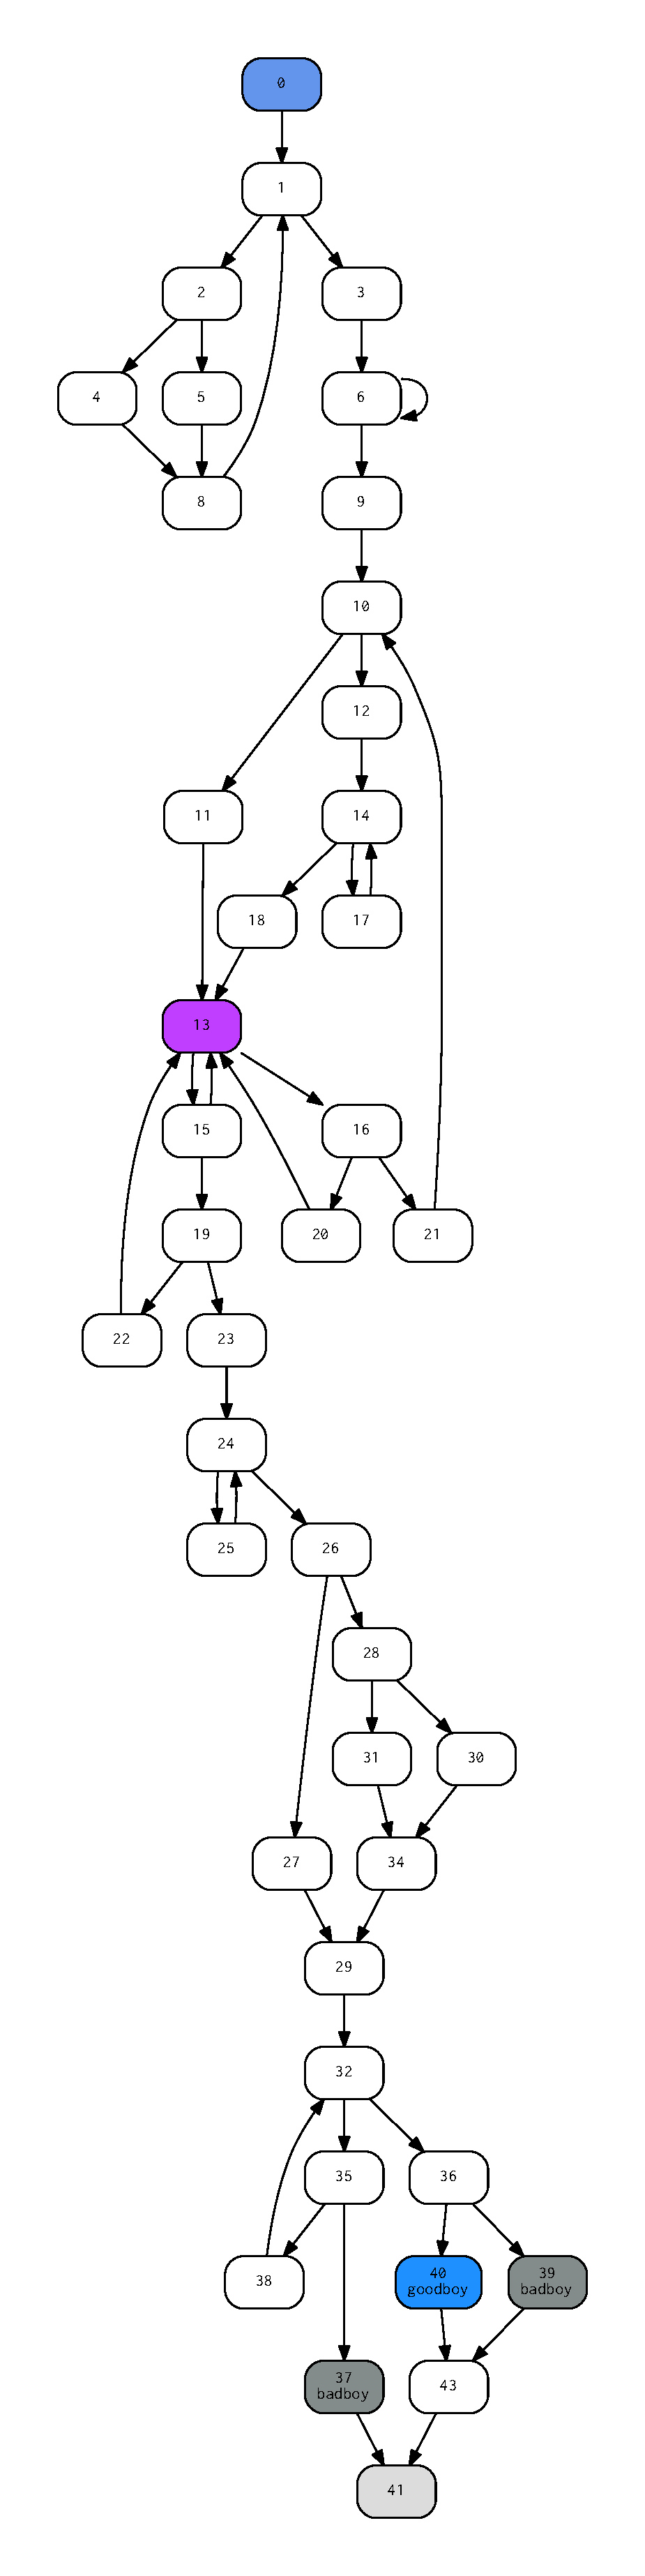
\includegraphics[height=1\textheight,keepaspectratio]{panda_cfg.pdf}
  \caption{Control flow graph}\label{fig:cfg}
\end{figure}

\section{Conclusion}
This challenge is very similar with the 


\printbibliography

\end{document}